\section{Introduction}
\frame{\tableofcontents[currentsection, hideothersubsections]}

\begin{frame}
\frametitle{Keyword definitions}
\begin{itemize}
  \item Autonomous robots (or agents)? \pause
    \begin{figure}
      \centering
      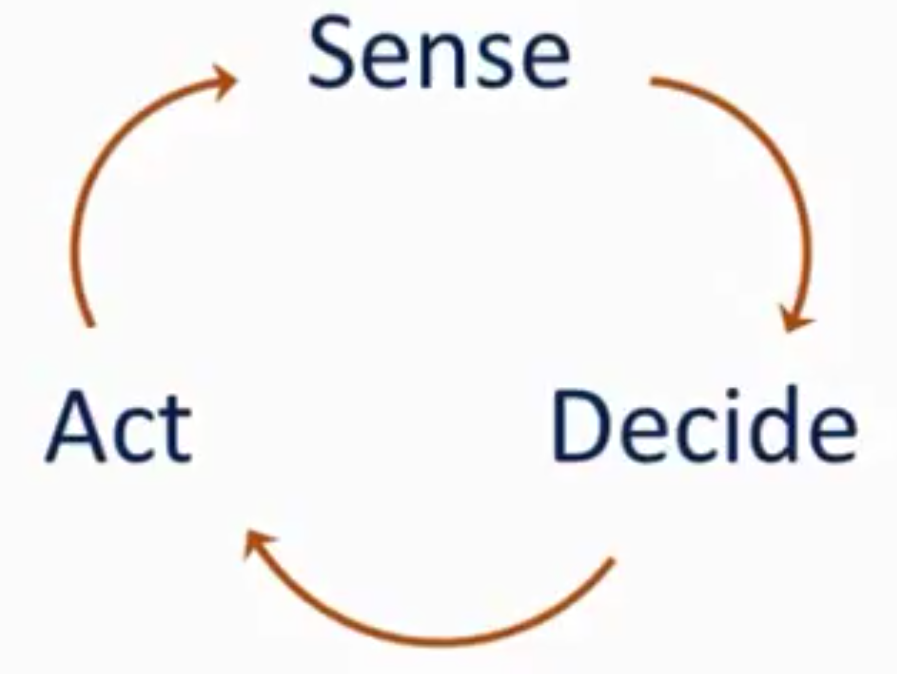
\includegraphics[scale=0.10]{sensePlanAct}
    \end{figure}
    \pause
  \begin{itemize}
    \item building \textbf{real} robots in \textbf{real} world is \textbf{real} hard, why?
  \end{itemize}
  \pause

  \item Artificial Intelligence? \pause
  \begin{itemize}
    \item planning (make sequential decisions) \pause
    \item learning (benefit from experience)
  \end{itemize}
  \pause

  \item Architecture for auto robots?
  \begin{itemize}
    \item provide the interplay between planning and learning
  \end{itemize}
  \pause

  \item Intro to ...?
  \begin{itemize}
    \item basic, foundation, simplistic setting, ...
    \item mostly pointers, top-down
  \end{itemize}
\end{itemize}
\end{frame}

\begin{frame}
\frametitle{Architecture Overview}
\begin{figure}
    \centering
    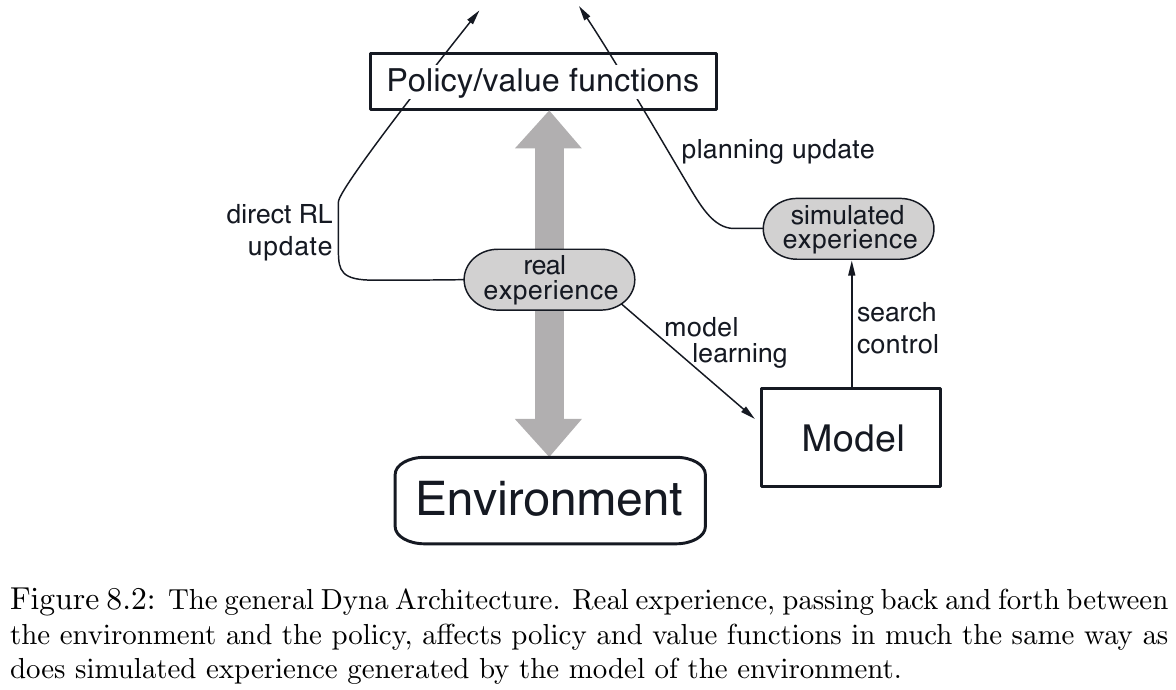
\includegraphics[scale=0.40]{dyna_rl_intro_p177}
\end{figure}
\end{frame}

\begin{frame}
\frametitle{Motivating examples}
\begin{itemize}
  \item a walking robot (UC Berkeley)
  \item a cart pole (TU Darmstat)
  \item a little dog (CMU, USC)
  \item an auto helicopter (Stanford)
\end{itemize}
\end{frame}
